\chapter{Curvilinear Coordinates} \label{sec:curvilinear2}
\label{chapter:curv}

\todoin{some obs from Applicable Differential Geometry}


\section{Curvilinear Coordinates}

The location of a point $P$ in space can be represented in many different 
 ways. Three systems commonly used in applications are the \emph{ rectangular
 cartesian system of Coordinates} $(x,y,z)$, the \emph{ cylindrical polar 
 system of Coordinates} $(r,\phi,z)$ and the 
 \emph{ spherical system of Coordinates} $(r,\varphi,\phi)$. 
 The last two are the best examples 
 of \emph{ orthogonal curvilinear} systems of coordinates 
 $(u_{1},u_{2},u_{3})$ . 



 

\begin{df}
    A function $\vector{u}:U \to V$ is called a (differentiable) \negrito{coordinate change} if 
        \begin{itemize}
     \item  $\vector{u}$ is bijective
     \item $\vector{u}$ is differentiable 
     \item $\D\vector{u}$ is invertible at every point.
    \end{itemize}
\end{df}

\begin{figure}[h]
 \centering
 \includegraphics[width=7cm]{./figs/coordinates.eps}
 % coordinates.eps: 0x0 pixel, 300dpi, 0.00x0.00 cm, bb=
 \caption{Coordinate System}
 \label{fig:coord2}
\end{figure}






%  Let $(u_{1},u_{2},u_{3})$ be the coordinates of $P$ in a general curvilinear 
%  system of coordinates. If the curves $u_{1}$, $u_{2}$, and $u_{3}$ are mutually 
%  perpendicular, the system $(u_{1},u_{2},u_{3})$ is an \emph{ orthogonal 
%  curvilinear system of Coordinates} .


In the tridimensional case, suppose that $(x, y, z)$ are expressible as single-valued functions $\vector{u}$ of the 
variables $(u_1, u_2, u_3)$. Suppose also that $(u_1, u_2, u_3)$ can be 
expressed as single-valued functions of $(x,y,z)$. 

Through each point $P:(a,b,c)$ of the space   we have three surfaces: $u_1 = c_1$, $u_2 = c_2$ and $u_3 = c_3$,  where the constants $c_i$ are given by  $c_i=u_i(a,b,c)$

If say $u_{2}$ and $u_{3}$ are held fixed and $u_{1}$ 
 is made to vary, a \emph{ path} results. Such path is called a $u_{1}$ 
 \emph{ curve}. $u_{2}$ and $u_{3}$ curves can be constructed in analogous
 manner. 
 
 \begin{center}
 \begin{tikzpicture}[x=(10:3cm),y=(90:3cm),z=(215:2.75cm),
  >=Triangle, 
  %*/.tip=Circle,
  domain=0:1, samples=50, variable=\t]
\coordinate (O) at (0,0,0); 

\shade [left color=blue, right color=blue!15!white, shading angle=135]
  (O) \foreach \x/\y in{\t/0,1/\t,1-\t/1,0/1-\t}{
     -- plot [smooth] (non-linear cs:x=\x, y=\y) };
\shade [left color=red, right color=red!15!white, shading angle=45]  
  (O) \foreach \x/\z in{\t/0,1/\t,1-\t/1,0/1-\t}{
     -- plot [smooth] (non-linear cs:x=\x, z=\z) };
\shade[left color=cyan, right color=cyan!15!white, shading angle=225] 
  (O) \foreach \y/\z in{\t/0,1/\t,1-\t/1,0/1-\t}{
     -- plot [smooth] (non-linear cs:y=\y, z=\z) };

\draw [thick, draw=blue, -*] (O) -- plot [domain=0:1.125, smooth] 
  (non-linear cs:x=\t) node [right] {$u_2$};
\draw [thick, draw=blue, -*] (O) -- plot [domain=0:1.125, smooth] 
  (non-linear cs:y=\t) node [above] {$u_3$};
\draw [thick, draw=blue, -*] (O) -- plot [domain=0:1.125, smooth] 
  (non-linear cs:z=\t) node [below] {$u_1$};

% \draw [thick, ->] (O) -- (5/4,0,0) node [at end, right] {$q_2$ axis};
% \draw [thick, ->] (O) -- (0,5/4,0) node [at end, above] {$q_3$ axis};
% \draw [thick, ->] (O) -- (0,0,5/4) node [at end, left]  {$q_1$ axis};

\node at (1/2,1/2,0) {$u_1=\mbox{const}$};
\node at (0,1/2,2/3) {$u_2=\mbox{const}$};
\node at (3/4,0,3/4) {$u_3=\mbox{const}$};
\end{tikzpicture}
 \end{center}

The system  $(u_1,u_2,u_3)$ is said to be a \negrito{curvilinear coordinate system}. 



\begin{exa}
 
The parabolic cylindrical coordinates are defined in terms of the
Cartesian coordinates by:
\begin{align*}
x &= \sigma \tau \\
y &= \frac{1}{2} \left( \tau^2 - \sigma^2 \right) \\
z &= z
\end{align*}

The constant surfaces are the plane 
\[z=z_1\] 
and the parabolic cylinders
\[2 y = \frac{x^2}{\sigma^2} - \sigma^2\]
and
\[2 y = -\frac{x^2}{\tau^2} + \tau^2\]
\end{exa}


 \begin{figure}[!h]
 \centering
 \includegraphics[width=8cm]{./figs/ParabolicCylindricalCoordinates.eps}
 % ParabolicCylindricalCoordinates.eps: 0x0 pixel, 300dpi, 0.00x0.00 cm, bb=
\end{figure}


\subsection*{Coordinates I}
The surfaces $u_2 = u_2(P)$ and $u_3 = u_3(P)$
 intersect in a curve, along which only $u_1$
varies.

\begin{center}
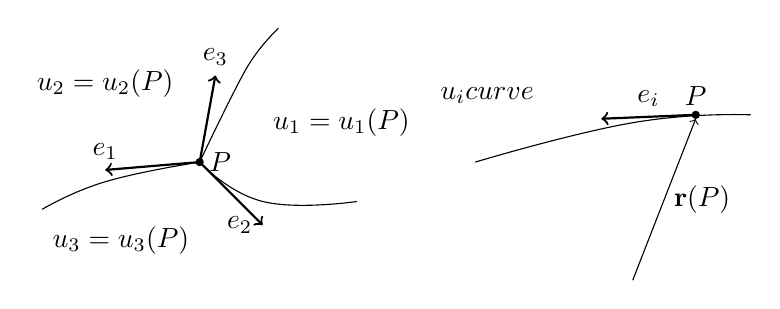
\begin{tikzpicture}
  \draw [->,thick] (0,0) -- (0.2,1.1) node [above] {$\versor e_3$};
  \draw [->,thick] (0,0) -- (.8,-.8) node [left] {$\versor e_2$};
  \draw [->,thick] (0,0) -- (-1.2,-.1) node [above] {$\versor e_1$};
  \fill (0,0) circle (1.5pt) node [right] {$P$};  
  \draw plot [smooth,tension=.6] coordinates {(0,0) (.6,1.2) (1,1.7)};
  \draw plot [smooth,tension=.8] coordinates {(0,0) (.8,-.5) (2,-.5)};
  \draw plot [smooth,tension=.8] coordinates {(0,0) (-1.2,-.25) (-2,-.6)}; 
  \node at (1.8,.5) {$u_1 = u_1(P)$};
  \node at (-1,-1) {$u_3 = u_3(P)$};
  \node at (-1.2,1) {$u_2 = u_2(P)$};
   
  \begin{scope}[shift={(3.5,0)}]
    \draw plot [smooth,tension=.8] coordinates {(0,0) (2,.5) (3.5,.6)};
%     \draw[->] (2,-1.5) -- (.8, .2) node[left,midway] {$\mathbf r(Q)$}; 
    \draw[->] (2,-1.5) -- (2.8,.55)node[right,midway] {$\mathbf r(P)$};   
%     \fill (2,-1.5) circle (1.5pt) node [right] {$O$};  
    \fill (2.8,.6) circle (1.5pt) node [above]  {$P$};
     \fill (.15, .62) circle (0.05pt) node [above]  {$u_i \text{ curve }$};
    \draw[->,thick] (2.8,.6) -- (1.6,.55) node [above,midway] {$\versor e_i$};
  \end{scope}     
\end{tikzpicture}
\end{center}
 
Let $\versor e_1$ be the unit vector tangential to the curve at $P$. Let $\versor e_2,\, \versor e_3$ be unit vectors
tangential to curves along which only $u_2, u_3$ vary.


Clearly 
\[\versor e_i=\dfrac{\partial \mathbf r}{\partial  u_1}/\norm{\dfrac{\partial \mathbf r}{\partial  u_i}}.\]
And if we define $h_i = |\partial \mathbf r/\partial  u_i|$ then
\begin{align*}
  \dfrac{\partial \mathbf r}{\partial  u_i} &= \versor e_i \cdot h_i
  \end{align*}

The quantities 
$h_i$ are often known as the \negrito{length scales} for the coordinate system.\\

% For an orthogonal system we must have $\versor e_i = \versor e^i$ (left diagram above). 
% Let $Q$ be a neighborhood point to $P$ on the curve along
% which only $u_i$ varies (right diagram above). 
% 
% We have
% \begin{align*}
%   \dfrac{\partial \mathbf r}{\partial  u_i}
%   &= \lim_{P \to Q}\dfrac{(\mathbf r(Q) - \mathbf r(P))}{\delta u_i}\\[.2cm]
%   &= \lim_{P \to Q} \dfrac{(\mathbf r(Q) - \mathbf r(P))}{PQ}\cdot \lim_{P \to Q}\left(\dfrac{PQ}{\delta u_i}\right)\\
%   &= \lim_{Q \to P} \dfrac{\vec{PQ}}{PQ} \cdot \lim_{P \to Q}\left(\dfrac{PQ}{\delta u_i}\right)\\
%   &= \versor e_i \cdot h_i
% \end{align*}
% 


\subsection*{Coordinates II}


Let $(\versor e^i,\versor e^2,\versor e^3)$ be unit vectors at $P$ in the directions normal to 
$u_1 = u_1(P),\,u_2 = u_2(P),u_3 = u_3(P)$
 respectively, such that $u_1, u_2, u_3$ increase in the directions $\versor e^1, \versor e^2,\hat  a_3.$ Clearly we must have
 \[
  \versor e^i = \nabla(u_i)/|\nabla u_i|
\]
% These vectors are tangent to the curves parametrized by $u_1, u_1, u_3$ respectively when the other two variables are being fixed.

\begin{df}
 If $(\versor e^1, \versor e^2,\versor e^3)$ are mutually orthogonal, the coordinate system is said to be an \negrito{orthogonal}
curvilinear coordinate system.
\end{df}

In an orthogonal system we have
\[
  \versor e_i = \versor e^i = \dfrac{\partial \mathbf r/\partial u_i}{|\partial \mathbf r/\partial u_i|}  = \nabla u_i / |\nabla u_i| \quad \mbox{ for $i=1,2,3$}
\]


So we associate to a  general curvilinear coordinate system  two sets of
basis vectors for every point:
\[\{\versor e_1,\versor e_2, \versor e_3\}\]
is the
\negrito{covariant basis}, and 
\[\{\versor e^1,
\versor e^2, \versor e^3\} \]
is the
\negrito{contravariant basis}. 

 \begin{figure}[h!]
 \centering
 \includegraphics[width=8.5cm]{./figs/bases.eps}
 % bases.eps: 0x0 pixel, 300dpi, 0.00x0.00 cm, bb=
\caption{Covariant and Contravariant Basis}
\end{figure}


% The covariant and contravariant
% basis vectors types have identical direction for orthogonal curvilinear
% coordinate systems, but as usual have inverted units with respect to
% each other.

Note the following important equality:
\[\versor e^i\cdot\versor e_j = \delta^i_j.\]


\begin{exa}
 \textbf{Cylindrical coordinates} $(r,\theta,z)$:
 \begin{align*}
  x &= r \cos \theta & r &= \sqrt{x^2 + y^2}\\
  y &= r \sin \theta & \theta &= \tan^{-1} \left( \dfrac{y}{x} \right)\\
  z &= z & z &= z
 \end{align*}
 \vspace{3mm}where $~0 \le \theta \le \pi~~$ if $~~y \ge 0~~$ and $~~\pi < \theta < 2\pi~~$ if $~~y < 0$
 
 For cylindrical coordinates $(r,\theta,z)$, and constants $\ssub{r}{0}$, $\ssub{\theta}{0}$ and $\ssub{z}{0}$, we see
from Figure \ref{fig:cylcoordsurf}
that the surface $r = \ssub{r}{0}$ is a cylinder of radius $\ssub{r}{0}$ centered along the $z$-axis, the surface
$\theta = \ssub{\theta}{0}$ is a half-plane emanating from the $z$-axis, and the surface $z = \ssub{z}{0}$ is a plane
parallel to the $xy$-plane.

\begin{figure}[h]
 \centering
 \subfloat[][$r = \ssub{r}{0}$]{
 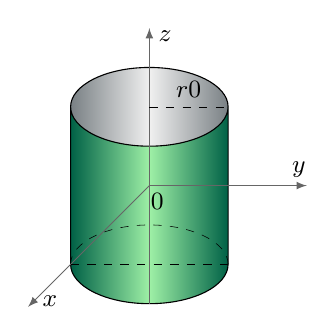
\begin{tikzpicture}
  \usetikzlibrary{arrows}
  \definecolor{insideo}{HTML}{798084}
  \definecolor{insidei}{HTML}{F0F0F0}
  \definecolor{outer}{HTML}{006146}
  \definecolor{inner}{HTML}{9EF0A6}
  \shade [left color=insideo,right color=insideo,middle color=insidei] (1,1) arc (0:180:1 and .5) --
   (-1,1) arc (180:360:1 and .5);
  \shadedraw [left color=outer,right color=outer,middle color=inner] (-1,-1) arc (180:360:1 and .5) -- (1,1) --
   (1,1) arc (360:180:1 and .5) -- (-1,-1);
  \draw (1,1) arc (0:180:1 and .5);
  \draw [dashed,line width=0.2pt] (1,-1) arc (0:180:1 and .5);
  \draw [black!60,line width=0.3pt,-latex] (0,0) -- (2,0,0);
  \draw [black!60,line width=0.3pt,-latex] (0,-1.5) -- (0,2,0);
  \draw [black!60,line width=0.3pt,-latex] (0,0) -- (0,0,4);
  \pgfputat{\pgfpointxyz{1.9}{0.2}{0}}{\pgfbox[center,center]{\small $y$}};
  \pgfputat{\pgfpointxyz{0.2}{1.9}{0}}{\pgfbox[center,center]{\small $z$}};
  \pgfputat{\pgfpointxyz{0.2}{0}{3.8}}{\pgfbox[center,center]{\small $x$}};
  \pgfputat{\pgfpointxyz{0.1}{-0.2}{0}}{\pgfbox[center,center]{\small $0$}};
  \draw [dashed,line width=0.2pt] (0,1) -- (1,1);
  \draw [dashed,line width=0.2pt] (-1,-1) -- (1,-1);
  \node [above] at (0.5,1) {\small $\ssub{r}{0}$};
 \end{tikzpicture}}
 \qquad\qquad
 \subfloat[][$\theta = \ssub{\theta}{0}$]{
 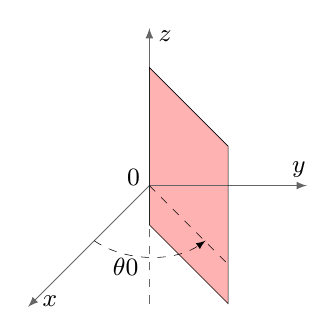
\begin{tikzpicture}
  \usetikzlibrary{arrows}
  \fill [red!30] (0,-.5) -- (1,-1.5) -- (1,.5) -- (0,1.5) -- (0,-.5);
  \draw [black!60,line width=0.3pt,-latex] (0,0) -- (2,0,0);
  \draw [black!60,line width=0.3pt,-latex] (0,-.5) -- (0,2,0);
  \draw [black!60,dashed,line width=0.3pt] (0,-1.5) -- (0,-.5);
  \draw [black!60,line width=0.3pt,-latex] (0,0) -- (0,0,4);
  \pgfputat{\pgfpointxyz{1.9}{0.2}{0}}{\pgfbox[center,center]{\small $y$}};
  \pgfputat{\pgfpointxyz{0.2}{1.9}{0}}{\pgfbox[center,center]{\small $z$}};
  \pgfputat{\pgfpointxyz{0.2}{0}{3.8}}{\pgfbox[center,center]{\small $x$}};
  \pgfputat{\pgfpointxyz{-0.2}{0.1}{0}}{\pgfbox[center,center]{\small $0$}};
  \draw [line width=0.2pt] (0,-.5) -- (1,-1.5) -- (1,.5) -- (0,1.5) -- (0,-.5);
  \draw [dashed,line width=0.2pt] (0,0) -- (1,-1);
  \draw [dashed,line width=0.2pt,-latex] (-0.7,-0.7) arc (225:315:1 and .7);
  \node [below] at (-0.3,-.8) {\small $\ssub{\theta}{0}$};
 \end{tikzpicture}}
 \qquad\qquad
 \subfloat[][$z = \ssub{z}{0}$]{
 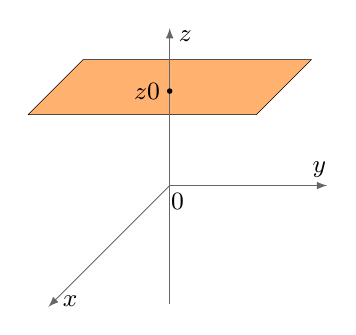
\begin{tikzpicture}
  \usetikzlibrary{arrows}
  \definecolor{planecolor}{HTML}{FFB270}
  \fill [planecolor] (-1.8,.9) -- (-1.1,1.6) -- (1.8,1.6) -- (1.1,.9) -- (-1.8,.9);
  \draw [line width=0.2pt] (-1.8,.9) -- (-1.1,1.6) -- (1.8,1.6) -- (1.1,.9) -- (-1.8,.9);
  \draw [black!60,line width=0.3pt,-latex] (0,0) -- (2,0,0);
  \draw [black!60,line width=0.3pt,-latex] (0,-1.5) -- (0,2,0);
  \draw [black!60,line width=0.3pt,-latex] (0,0) -- (0,0,4);
  \pgfputat{\pgfpointxyz{1.9}{0.2}{0}}{\pgfbox[center,center]{\small $y$}};
  \pgfputat{\pgfpointxyz{0.2}{1.9}{0}}{\pgfbox[center,center]{\small $z$}};
  \pgfputat{\pgfpointxyz{0.2}{0}{3.8}}{\pgfbox[center,center]{\small $x$}};
  \pgfputat{\pgfpointxyz{0.1}{-0.2}{0}}{\pgfbox[center,center]{\small $0$}};
  \fill (0,1.2) circle (1pt);
  \node [left] at (0,1.2) {\small $\ssub{z}{0}$};
 \end{tikzpicture}}
 \caption[]{\quad Cylindrical coordinate surfaces}
 \label{fig:cylcoordsurf}
\end{figure}

The unit vectors $\hat r, \hat \theta,\hat k$ at any point $P$ are perpendicular to the surfaces $r =$ constant, $\theta =$ constant, $z =$ constant
 through $P$ in the directions of increasing $r, \theta, z$. Note that the direction of the unit vectors $\hat r,\hat \theta$ vary from point to point, unlike the corresponding Cartesian unit vectors.

\end{exa}



\section{Line and Volume Elements in Orthogonal Coordinate Systems}



\begin{definition}[Line Element]
Since $\mathbf r = \mathbf r(u_1,u_2,u_3)$,
the \emph{line element}
$\d \mathbf r$ is given by
\begin{align*}
  \d\mathbf r 
  &= \dfrac{\partial \mathbf r}{\partial u_1} \,\d u_1 
  + \dfrac{\partial \mathbf r}{\partial u_2} \,\d u_2 
  + \dfrac{\partial \mathbf r}{\partial u_3} \,\d u_3\\
  &= h_1\d u_1\versor {e_1}
  +  h_2\d u_2\versor {e_2}
  + h_3\d u_3\versor{e_3}
\end{align*}
\end{definition}

If the system is orthogonal, then it follows that
\[
  (\d s)^2 = (\d \mathbf r)\cdot  (\d \mathbf r) = h_1^2(\d u_1)^2 + 
  h_2^2(\d u_2)^2 +h_3^2(\d u_3)^2 
\]
In what follows we will assume we have an orthogonal system so that
\[
  \versor e_i = \versor e^i = \dfrac{\partial \mathbf r/\partial u_i}{|\partial \mathbf r/\partial u_i|}  = \nabla u_i / |\nabla u_i| \quad \mbox{ for $i=1,2,3$}
\]
In particular, line elements along curves of intersection of $u_i$ surfaces have lengths $h_1\d u_1,\, h_2\d u_2,\, h_3\d u_3$ respectively.\\


\begin{definition}[Volume Element]
In $\bbR^3$, the volume element is given by 
\[\d V = \dx\,\dy\,\dz.\]
In a coordinate systems
$x=x(u_1,u_2,u_3), y=y(u_1,u_2,u_3), z=z(u_1,u_2,u_3)$, the volume element  is:
\[\d V = \left|\dfrac{\partial (x,y,z)}{\partial (u_1,u_2,u_3)}\right|\,\d u_1\,\d u_2\,\d u_3.\]
\end{definition}


\begin{prop} In an orthogonal system we have
 \begin{align*}
  \d V &= (h_1\d u_1)(h_2 \d u_2)(h_3 \d u_3)\\
  &= h_1h_2h_3\,\d u_1\d u_2\d u_3
\end{align*}
\end{prop}


% \begin{center}
% \includegraphics[width=6cm]{fig20.jpg}	
% \end{center}



In this section we find the expression of the line and volume elements in some classics orthogonal coordinate systems.

 \textbf{(i) Cartesian Coordinates $(x,y,z)$}
\begin{align*}
  \d V &= \d x\d y \d z\\
   \d \mathbf r &= \d x\hat i + \d y \hat j + \d z \hat k\\
(\d s)^2  &= (\d\mathbf r)\cdot(\d \mathbf r) = (\d x)^2 + (\d y)^2 + (\d z)^2
\end{align*}


\textbf{(ii) Cylindrical polar coordinates $(r,\theta,z)$}
The coordinates are related to Cartesian by 
\[
  x = r\cos \theta,\, y = r\sin \theta,\, z = z
\]

% \begin{center}
% \includegraphics[width=7cm]{fig21.jpg}	
% \end{center}

We have that $(\d s)^2 = (\d x)^2 + (\d y)^2 + (\d z)^2$, but we can write 
\begin{align*}
  \d x &= \left(\dfrac{\partial x}{\partial r}\right)\,\d r + \left(\dfrac{\partial x}{\partial \theta}\right)\, \d \theta + \left(\dfrac{\partial x}{\partial z}\right)\,\d z\\
  &= (\cos \theta)\,\d r  - (r\sin \theta)\,\d \theta \\
  \intertext{and}
  \d y &= \left(\dfrac{\partial y}{\partial r}\right)\,\d r + \left(\dfrac{\partial y}{\partial \theta}\right)\, \d \theta + \left(\dfrac{\partial y}{\partial z}\right)\,\d z\\
  &= (\sin \theta)\,\d r + (r\cos\theta)\d \theta
\end{align*}
Therefore we have 
\begin{align*}
  (\d s)^2 &= (\d x)^2 + (\d y)^2 + (\d z)^2\\
  &= \dots = (\d r)^2 + r^2(\d\theta)^2 + (\d z)^2
\end{align*}
Thus we see that for this coordinate system, 
the length scales are 
\[
  h_1 = 1,\, h_2 = r,\, h_3 = 1
\]
and the element of volume is 
\[
  d V = r \,\d r\d \theta \d z
\]

\textbf{(iii) Spherical Polar coordinates $(r,\phi,\theta$)}
In this case the relationship between the coordinates is 
\[
  x = r \sin \phi \cos\theta;\; y = r\sin\phi\sin\theta;\; z = r\cos\phi
\]
% \begin{center}
% \includegraphics[width=8.5cm]{fig22.png}	
% \end{center}
Again, we have that $(\d s)^2 = (\d x)^2 + (\d y)^2 + (\d z)^2$ and we know that 
\begin{align*}
  \d x 
  &= \dfrac{\partial x}{\partial r}\d r + \dfrac{\partial x}{\partial \theta}\d \theta + \dfrac{\partial x}{\partial \phi}\d \phi\\
  &= (\sin\phi\cos\theta)\d r + (-r\sin\phi\sin\theta)\d \theta + r\cos\phi\cos\theta \d \phi 
  \intertext{and}
  \d y 
  &= \dfrac{\partial y}{\partial r}\d r + \dfrac{\partial y}{\partial \theta}\d \theta + \dfrac{\partial y}{\partial \phi}\d \phi\\
  &= \sin\phi\sin\theta \d r + r\sin\phi\cos\theta \d \theta + r\cos\phi\sin\theta \d \phi 
  \intertext{together with}
  \d z 
  &= \dfrac{\partial z}{\partial r}\d r + \dfrac{\partial z}{\partial \theta}\d \theta + \dfrac{\partial z}{\partial \phi}\d \phi\\
  &= (\cos\phi)\d r - (r\sin\phi)\d \phi
\end{align*}
Therefore in this case, we have (after some work)
\begin{align*}
  (\d s)^2 &= (\d x)^2 + (\d y)^2 + (\d z)^2\\
  &= \dots = (\d r)^2 + r^2(\d \phi)^2 + r^2\sin^2\phi(\d \theta)^2
\end{align*}
Thus the length scales are 
\[
  h_1 = 1,\, h_2 = r,\, h_3 = r\sin\phi 
\]
and the volume element is 
\[
  \d V = r^2\sin\phi\,\d r\d \phi \d \theta
\]



\begin{exa}
\emph{Find the volume and surface area of a sphere of 
radius $a$, and also find the surface area of a cap of the sphere that subtends on angle $\alpha$ at the centre of the sphere.}

\[
  d V = r^2 \sin\phi\,\d r \d \phi \d \theta 
\]
and an element of surface of a sphere of radius $a$ is (by removing $h_1\d u_1 = \d r$):
\[
  \d S = a^2 \sin \phi \,\d \phi\,\d \theta 
\]
$\therefore$ total volume is 
\begin{align*}
  \int_V \,\d V 
  &= \int_{\theta=0}^{2\pi}\int_{\phi =0}^\pi \int_{r=0}^a r^2\sin\phi\, \d r \d \phi \d \theta \\
  &= 2\pi[-\cos\phi]_0^\pi \int_0^a r^2\,\d r\\
  &= 4\pi a^3/3\;
\end{align*}

Surface area is 
\begin{align*}
  \int_S \,\d S 
  &= \int_{\theta=0}^{2\pi} \int_{\phi =0}^\pi a^2\sin\phi \,\d\phi\,\d\theta\\
  &= 2\pi a^2[-\cos\phi]_0^\pi\\
  &= 4\pi a^2 \; 
\end{align*}

Surface area of cap is
\begin{align*}
  \int_{\theta=0}^{2\pi}\int_{\phi=0}^\alpha 
  a^2\sin\phi \,\d\phi\,\d \theta
  &= 2\pi a^2[-\cos\phi]_0^\alpha\\
  &= 2\pi a^2(1-\cos\alpha)
\end{align*}
\end{exa}


\section{Gradient in Orthogonal Curvilinear Coordinates}
Let 
\[
  \nabla \Phi = \lambda_1\versor e_1 + \lambda_2\versor e_2 + \lambda_3\versor e_3
\]
in a general coordinate system, where $\lambda_1,\lambda_2,\lambda_3$ are to be found. 
Recall that the element of length is given by 
\[
  \d \mathbf r = h_1\d u_1\versor e_1 + h_2\d u_2\versor e_2 + h_3\d u_3\versor e_3
\]
Now 
\begin{align*}
  \d \Phi &= \dfrac{\partial \Phi}{\partial u_1}\d u_1 + \dfrac{\partial \Phi}{\partial u_2}\d u_2 + \dfrac{\partial \Phi}{\partial u_3}\d u_3\\
  &= \dfrac{\partial \Phi}{\partial x}\d x + \dfrac{\partial \Phi}{\partial  y}\d y + \dfrac{\partial \Phi}{\partial z}\d z\\
  &= (\nabla \Phi)\cdot \d \mathbf r 
\end{align*}

But, using our expressions for $\nabla \Phi$ and $\d \mathbf r$ above:
\[
  (\nabla \Phi)\cdot \d \mathbf r = \lambda_1h_1\d u_1 + \lambda_2h_2\d u_2 + \lambda_3h_3\d u_3
\]
and so we see that 
\[
  h_i\lambda_i = \dfrac{\partial \Phi}{\partial u_i} \mbox{ ($i = 1,2,3$)}
\]
Thus we have the result that 

\begin{prop}[Gradient in Orthogonal Curvilinear Coordinates]
 \[
  \nabla \Phi = \dfrac{\versor e_1}{h_1}\dfrac{\partial \Phi}{\partial u_1} + \dfrac{\versor e_2}{h_2}\dfrac{\partial \Phi}{\partial u_2} + \dfrac{\versor e_3}{h_3}\dfrac{\partial \Phi}{\partial u_3}
\]
\end{prop}


This proposition allows us to write down $\nabla$ easily for other coordinate systems. 


\textbf{(i) Cylindrical polars $(r,\theta,z)$}
Recall that $h_1 = 1,\, h_2 = r,\, h_3 = 1$. Thus
\[
  \nabla = \hat r \dfrac{\partial}{\partial r} + \dfrac{\hat 
  \theta}{r}\dfrac{\partial }{\partial \theta} + \hat z \dfrac{\partial }{\partial z}
\]

\textbf{(ii) Spherical Polars $(r,\phi,\theta)$}
We have $h_1 = 1,\, h_2 = r,\, h_3 = r\sin\phi$, and so 
\[
  \nabla = \hat r \dfrac{\partial }{\partial r} + \dfrac{\hat \phi}{r}\dfrac{\partial }{\partial \phi} + \dfrac{\hat \theta}{r \sin\phi}\dfrac{\partial }{\partial \theta}
\]

\subsection{Expressions for Unit Vectors}

From the expression for $\nabla$ we have just derived, it is easy to see that 
\[
  \versor e_i = h_i \nabla u_i
\]
Alternatively, since the unit vectors are orthogonal, if we know two unit vectors we can find the third from the relation
\[
  \versor e_1 = \versor e_2 \times \versor e_3 = h_2h_3(\nabla u_2 \times \nabla u_3)
\]
and similarly for the other components, by permuting in a cyclic fashion.


\section{Divergence in Orthogonal Curvilinear Coordinates}

Suppose we have a vector field
\[
  \mathbf A = A_1 \versor e_1 + A_2 \versor e_2 + A_3 \versor e_3
\]
Then consider 
\begin{align*}
  \nabla \cdot (A_1 \versor e_1) 
  &= \nabla \cdot [A_1h_2h_3(\nabla u_2 \times \nabla u_3)]\\
  &= A_1h_2h_3 \nabla \cdot (\nabla u_2 \times \nabla u_3) + \nabla(A_1h_2h_3)\cdot \dfrac{\versor e_1}{h_2h_3}
\end{align*}
using the results established just above. Also we know that 
\[
  \nabla\cdot (\mathbf B \times \mathbf C) = \mathbf C \cdot \mathrm{curl}\,\mathbf B - \mathbf B \cdot \mathrm{curl}\,\mathbf C
\]
and so it follows that 
\[
  \nabla\cdot(\nabla u_2 \times \nabla u_3) = (\nabla u_3)\cdot \mathrm{curl}(\nabla u_2) - (\nabla u_2)\cdot \mathrm{curl}(\nabla u_3) = 0
\]
since the curl of a gradient is always zero. 
Thus we are left with
\[
  \nabla \cdot (A_1\versor e_1) = \nabla (A_1h_2h_3) \cdot \dfrac{\versor e_1}{h_2h_3} = \dfrac{1}{h_1h_2h_3}\dfrac{\partial }{\partial u_1} (A_1h_2h_3)
\]
We can proceed in a similar fashion for the other components, and establish that 

\begin{prop}[Divergence in Orthogonal Curvilinear Coordinates]
 
\[
 \nabla \cdot \mathbf A = \dfrac{1}{h_1h_2h_3}\left[\dfrac{\partial }{\partial u_1}(h_2h_3 A_1) + \dfrac{\partial }{\partial u_2}(h_3h_1 A_2) + \dfrac{\partial }{\partial u_3}(h_1h_2A_3)\right]
\]
\end{prop}

Using the above proposition is now  easy to write down  the divergence in other coordinate systems. 


\textbf{(i) Cylindrical polars $(r,\theta,z)$}

Since  $h_1 = 1,\, h_2 = r,\, h_3 = 1$  using the above formula we have :
\begin{align*}
  \nabla \cdot \mathbf A 
  &= \dfrac{1}{r}\left[\dfrac{\partial }{\partial r}(r A_1) + \dfrac{\partial }{\partial \theta}(A_2) + \dfrac{\partial }{\partial z}(r A_3)\right]\\[.2cm]
  &= \dfrac{\partial A_1}{\partial r} + \dfrac{A_1}{r} + \dfrac{1}{r}\dfrac{\partial A_2}{\partial \theta} +\dfrac{\partial A_3}{\partial z}
\end{align*}

\textbf{(ii) Spherical polars $(r,\phi,\theta)$}

We have $h_1 = 1,\, h_2 = r,\, h_3 = r\sin\phi$. So
\[
  \nabla \cdot \mathbf A = \dfrac{1}{r^2\sin\phi} \left[\dfrac{\partial }{\partial r}(r^2 \sin\phi A_1) + \dfrac{\partial }{\partial \phi}(r\sin\phi A_2) + \dfrac{\partial }{\partial \theta}(rA_3)\right]
\]


\section{Curl in Orthogonal Curvilinear Coordinates}

We will calculate the curl of the first component of $\mathbf A$:
\begin{align*}
  \nabla \times (A_1 \versor e_1)
  &= \nabla \times (A_1h_1\nabla u_1)\\[.2cm]
  &= A_1h_2\nabla \times (\nabla u_1) + 
  \nabla(A_1h_1) \times \nabla u_1\\[.2cm]
  &= 0 + \nabla (A_1h_1) \times \nabla u_1\\[.2cm]
  &= \left[\dfrac{\versor e_1}{h_1}\dfrac{\partial }{\partial u_1}(A_1h_1) + \dfrac{\versor e_2}{h_2}\dfrac{\partial }{\partial u_2}(A_1h_1) + \dfrac{\versor e_3}{h_3}\dfrac{\partial }{\partial u_3}(A_1h_1)\right] \times \dfrac{\versor e_1}{h_1}\\[.2cm]
  &= \dfrac{\versor e_2}{h_1h_3}\dfrac{\partial }{\partial u_3}(h_1A_1) - \dfrac{\versor e_3}{h_1h_2}\dfrac{\partial }{\partial u_2}(h_1A_1)
\end{align*}
(since $\versor e_1 \times \versor e_1 = 0,\, \versor e_2 \times \versor e_1 = -\versor e_3,\, \versor e_3 \times \versor e_1 = \versor e_2$). 

We can obviously find curl$(A_2\versor e_2)$ and curl$(A_3\versor e_3)$ in a similar way. 
These can be shown to be 
\begin{align*}
  \nabla \times (A_2 \versor e_2) &= 
  \dfrac{\versor e_3}{h_2h_1}\dfrac{\partial }{\partial u_1}(h_2A_2) - \dfrac{\versor e_1}{h_2h_3}\dfrac{\partial }{\partial u_3}(h_2A_2)\\
    \nabla \times (A_3 \versor e_3) &= 
  \dfrac{\versor e_1}{h_3h_2}\dfrac{\partial }{\partial u_2}(h_3A_3) - \dfrac{\versor e_2}{h_3h_1}\dfrac{\partial }{\partial u_1}(h_3A_3)
\end{align*}
Adding these three contributions together, we find we can write this in the form of a determinant as 

\begin{prop}[Curl in Orthogonal Curvilinear Coordinates]
\[  \mathrm{curl}\,\mathbf A = \dfrac{1}{h_1h_2h_3}
  \begin{vmatrix}
  h_1\versor e_1 & h_2 \versor e_2 & h_3\versor e_3\\
  \partial _{u_1} &\partial _{u_2} &\partial _{u_3}\\
  h_1A_1 & h_2A_2 & h_3A_3
  \end{vmatrix}
\]

\end{prop}

It's then straightforward to write down the expressions of the  curl in various orthogonal coordinate systems.

\textbf{(i) Cylindrical polars}
\[
  \mathrm{curl}\,\mathbf A = 
  \dfrac{1}{r}
  \begin{vmatrix}
  \hat r & r\hat \theta & \hat z\\
  \partial _r & \partial _\theta &\partial _z\\
  A_1 & rA_2 & A_3	
  \end{vmatrix}
\]

\textbf{(ii) Spherical polars}
\[
  \mathrm{curl}\,\mathbf A = \dfrac{1}{r^2\sin\phi} 
  \begin{vmatrix}
  	\hat r & r\hat \phi & r\sin\phi \hat \theta\\
  	\partial _r & \partial _\phi & \partial _\theta\\
  	A_1 & rA_2 & r\sin\phi A_3
  \end{vmatrix}
\]

\section{The Laplacian in Orthogonal Curvilinear Coordinates}
From the formulae already established for the gradient and the  divergent, we can see that 

\begin{prop}[The Laplacian in Orthogonal Curvilinear Coordinates]
\begin{align*}
  \nabla^2\Phi 
  &= \nabla \cdot(\nabla \Phi)\\
  &= \dfrac{1}{h_1h_2h_3}\left[\dfrac{\partial }{\partial u_1}(h_2h_3\dfrac{1}{h_1}\dfrac{\partial \Phi}{\partial u_1}) + \dfrac{\partial }{\partial u_2}(h_3h_1\dfrac{1}{h_2}\dfrac{\partial \Phi}{\partial u_2}) + \dfrac{\partial }{\partial u_3}(h_1h_2\dfrac{1}{h_3}\dfrac{\partial \Phi}{\partial u_3})\right]
\end{align*}
\end{prop}

% The formula can then be used to calculate the Laplacian for various coordinate systems.

\textbf{(i) Cylindrical polars $(r,\theta,z)$}
\begin{align*}
  \nabla^2\Phi 
  &= \dfrac{1}{r}\left[\dfrac{\partial }{\partial r}\left(r\dfrac{\partial \Phi}{\partial r}\right) + \dfrac{\partial }{\partial \theta}\left(\dfrac{1}{r}\dfrac{\partial \Phi}{\partial \theta}\right) + \dfrac{\partial }{\partial z}\left(r \dfrac{\partial \Phi}{\partial z}\right)\right]\\[.2cm]
  &= \dfrac{\partial ^2\Phi}{\partial r^2} + \dfrac{1}{r}\dfrac{\partial \Phi}{\partial r} + \dfrac{1}{r^2}\dfrac{\partial ^2\Phi}{\partial \theta^2} + \dfrac{\partial ^2\Phi}{\partial z^2}
\end{align*}

\textbf{(ii) Spherical polars $(r,\phi,\theta)$}
\begin{align*}
  \nabla^2\Phi 
  &= \dfrac{1}{r^2\sin\phi}
  \left[\dfrac{\partial }{\partial r}\left(r^2\sin\phi \dfrac{\partial \Phi}{\partial r}\right) + \dfrac{\partial }{\partial \phi}\left(\sin\phi \dfrac{\partial \Phi}{\partial \phi}\right) + \dfrac{\partial }{\partial \theta}\left(\dfrac{1}{\sin\phi}\dfrac{\partial \Phi}{\partial \theta}\right)\right]\\[.2cm]
  &= \dfrac{\partial ^2\Phi}{\partial r^2} + \dfrac{2}{r}\dfrac{\partial \Phi}{\partial r} + \dfrac{\cot \phi}{r^2}\dfrac{\partial \Phi}{\partial \phi} + \dfrac{1}{r^2}\dfrac{\partial ^2\Phi}{\partial \phi^2} + \dfrac{1}{r^2\sin^2\phi}\dfrac{\partial ^2\Phi}{\partial \theta^2}
\end{align*}



\begin{exa}
 In Example \ref{exa:laplposition} we showed that $\nabla \norm{\textbf{r}}^2 = 2\,\textbf{r}$ and
 $\Delta \norm{\textbf{r}}^2 = 6$, where $\textbf{r}(x,y,z) = x\,\textbf{i} + y\,\textbf{j} + z\,\textbf{k}$ in
 Cartesian coordinates. Verify that we get the same answers if we switch to spherical coordinates.\vspace{1mm}
 \par\noindent \emph{Solution:} Since $\norm{\textbf{r}}^2 = x^2 + y^2 + z^2 = \rho^2$ in spherical
 coordinates, let $F(\rho,\theta,\phi) = \rho^2$ (so that $F(\rho,\theta,\phi) =
 \norm{\textbf{r}}^2$). The gradient of $F$ in spherical coordinates is
 \begin{align*}
  \nabla F ~&=~ \frac{\partial F}{\partial \rho}\,\textbf{e}_{\rho} ~+~
   \frac{1}{\rho \sin \phi}\,\frac{\partial F}{\partial \theta}\,\textbf{e}_{\theta} ~+~
   \frac{1}{\rho}\,\frac{\partial F}{\partial \phi}\,\textbf{e}_{\phi}\\
   &=~ 2\rho\,\textbf{e}_{\rho} ~+~ \frac{1}{\rho \sin \phi}\,(0)\,\textbf{e}_{\theta} ~+~
    \frac{1}{\rho}\,(0)\,\textbf{e}_{\phi}\\
   &=~ 2\rho\,\textbf{e}_{\rho} ~=~ 2\rho\,\frac{\textbf{r}}{\norm{\textbf{r}}} ~,~\text{as we showed earlier, so}\\
   &=~ 2\rho\,\frac{\textbf{r}}{\rho} ~=~ 2\,\textbf{r} ~,~\text{as expected. And the Laplacian is}\\
  \Delta\,F ~&=~ \frac{1}{\rho^2}\,\frac{\partial}{\partial \rho} \left( \rho^2 \,
   \frac{\partial F}{\partial \rho} \right) ~+~ \frac{1}{\rho^2 \sin^2 \phi}\,\frac{\partial^2 F}{\partial \theta^2} ~+~
   \frac{1}{\rho^2 \sin \phi}\,\frac{\partial}{\partial \phi} \left( \sin \phi \,\frac{\partial F}{\partial \phi}
   \right)\\
   &=~ \frac{1}{\rho^2}\,\frac{\partial}{\partial \rho} ( \rho^2 \,2\rho ) ~+~ \frac{1}{\rho^2 \sin \phi}\,(0) ~+~
    \frac{1}{\rho^2 \sin \phi}\,\frac{\partial}{\partial \phi} \left( \sin \phi \,(0) \right)\\
   &=~ \frac{1}{\rho^2}\,\frac{\partial}{\partial \rho} ( 2\rho^3 ) ~+~ 0 ~+~ 0\\
   &=~ \frac{1}{\rho^2}\,(6\rho^2 ) ~=~ 6 ~,~\text{as expected.}
 \end{align*}
\end{exa}


\begin{table}[h!]
 \begin{tabular}{ccl}
  \hline \rule{0pt}{4ex}    
  $\nabla \Phi$& =&$ \displaystyle\dfrac{\versor e_1}{h_1}\dfrac{\partial \Phi}{\partial u_1} + \dfrac{\versor e_2}{h_2}\dfrac{\partial \Phi}{\partial u_2} + \dfrac{\versor e_3}{h_3}\dfrac{\partial \Phi}{\partial u_3}$\\
$ \nabla \cdot \mathbf A$& =&$  \displaystyle\dfrac{1}{h_1h_2h_3}\left[\dfrac{\partial }{\partial u_1}(h_2h_3 A_1) + \dfrac{\partial }{\partial u_2}(h_3h_1 A_2) + \dfrac{\partial }{\partial u_3}(h_1h_2A_3)\right]$\\
$\mathrm{curl}\,\mathbf A$& =& $   \displaystyle\dfrac{1}{h_1h_2h_3}
  \begin{vmatrix}
  h_1\versor e_1 & h_2 \versor e_2 & h_3\versor e_3\\
  \partial _{u_1} &\partial _{u_2} &\partial _{u_3}\\
  h_1A_1 & h_2A_2 & h_3A_3
  \end{vmatrix}$\\
  $\nabla^2\Phi$  &=& $ \displaystyle\dfrac{1}{h_1h_2h_3}\left[\dfrac{\partial }{\partial u_1}(h_2h_3\dfrac{1}{h_1}\dfrac{\partial \Phi}{\partial u_1}) + \dfrac{\partial }{\partial u_2}(h_3h_1\dfrac{1}{h_2}\dfrac{\partial \Phi}{\partial u_2}) + \dfrac{\partial }{\partial u_3}(h_1h_2\dfrac{1}{h_3}\dfrac{\partial \Phi}{\partial u_3})\right]$   \rule{0pt}{4ex}  \\
   \hline 
 \end{tabular}
\caption{Vector operators in orthogonal curvilinear coordinates $u_ 1 , u_ 2 , u_ 3.$}
\end{table}

\section{Examples of  Orthogonal Coordinates}

\paragraph{Spherical Polar Coordinates} 
\((r, \phi, \theta)\in[0,\infty)\times[0,\pi]\times[0,2\pi)\) 
\begin{align}
x&=r\sin\phi\cos\theta \\
y&=r\sin\phi\sin\theta \\
z&=r\cos\phi
\end{align}
The scale factors for the Spherical Polar Coordinates are:
\begin{align}
h_1&=1 \\
h_2&=r \\
h_3&=r\sin\phi
\end{align}
\paragraph{Cylindrical Polar Coordinates} 

\((r, \theta, z)\in[0,\infty)\times[0,2\pi)\times(-\infty,\infty)\)
\begin{align}
x&=r\cos\theta \\
y&=r\sin\theta \\
z&=z
\end{align}
The scale factors for the Cylindrical Polar Coordinates are:

\begin{align}
h_1&=h_3=1 \\
h_2&=r
\end{align}
\paragraph{Parabolic Cylindrical
Coordinates} 

\((u, v, z)\in(-\infty,\infty)\times[0,\infty)\times(-\infty,\infty)\)
\begin{align}
x&=\frac{1}{2}(u^2-v^2)\\
y&=uv\\
z&=z
\end{align}
The scale factors for the Parabolic Cylindrical
Coordinates are:

\begin{align}
h_1&=h_2=\sqrt{u^2+v^2} \\
h_3&=1
\end{align}
\paragraph{Paraboloidal Coordinates} 

\((u, v, \theta)\in[0,\infty)\times[0,\infty)\times[0,2\pi)\)

\begin{align}
x&=uv\cos\theta\\
y&=uv\sin\theta\\
z&=\frac{1}{2}(u^2-v^2)
\end{align}
The scale factors for the Paraboloidal Coordinates are:
\begin{align}
h_1&=h_2=\sqrt{u^2+v^2} \\
h_3&=uv
\end{align}
\paragraph{Elliptic Cylindrical
Coordinates} 

\((u, v, z)\in[0,\infty)\times[0,2\pi)\times(-\infty,\infty)\)
\begin{align}
x&=a\cosh u \cos v\\
y&=a\sinh u \sin v\\
z&=z
\end{align}
The scale factors for the Elliptic Cylindrical
Coordinates are:

\begin{align}
h_1&=h_2=a\sqrt{\sinh^2u+\sin^2v} \\
h_3&=1
\end{align}
\paragraph{Prolate Spheroidal Coordinates} 

\((\xi, \eta, \theta)\in[0,\infty)\times[0,\pi]\times[0,2\pi)\) 
\begin{align}
x&=a\sinh\xi\sin\eta\cos\theta\\
y&=a\sinh\xi\sin\eta\sin\theta\\
z&=a\cosh\xi\cos\eta
\end{align}
The scale factors for the Prolate Spheroidal
Coordinates are:
\begin{align}
h_1&=h_2=a\sqrt{\sinh^2\xi+\sin^2\eta} \\
h_3&=a\sinh\xi\sin\eta
\end{align}
\paragraph{Oblate Spheroidal Coordinates} 
\((\xi, \eta, \theta)\in[0,\infty)\times\left[-\frac{\pi}{2},\frac{\pi}{2}\right]\times[0,2\pi)\)
\begin{align}
x&=a\cosh\xi\cos\eta\cos\theta\\
y&=a\cosh\xi\cos\eta\sin\theta\\
z&=a\sinh\xi\sin\eta
\end{align}
The scale factors for the Oblate Spheroidal
Coordinates are:

\begin{align}
h_1&=h_2=a\sqrt{\sinh^2\xi+\sin^2\eta} \\
h_3&=a\cosh\xi\cos\eta
\end{align}
\paragraph{Ellipsoidal Coordinates} \begin{align}
& (\lambda, \mu, \nu)\\
& \lambda < c^2 < b^2 < a^2,\\
& c^2 < \mu < b^2 < a^2,\\
& c^2 < b^2 < \nu < a^2,
\end{align}

\(\frac{x^2}{a^2 - q_i} + \frac{y^2}{b^2 - q_i} + \frac{z^2}{c^2 - q_i} = 1\)
where \((q_1,q_2,q_3)=(\lambda,\mu,\nu)\) 

The scale factors for the Ellipsoidal
Coordinates are:
\(h_i=\frac{1}{2} \sqrt{\frac{(q_j-q_i)(q_k-q_i)}{(a^2-q_i)(b^2-q_i)(c^2-q_i)}}\)

\paragraph{Bipolar Coordinates}
\((u,v,z)\in[0,2\pi)\times(-\infty,\infty)\times(-\infty,\infty)\)
\begin{align}
x&=\frac{a\sinh v}{\cosh v - \cos u}\\
y&=\frac{a\sin u}{\cosh v - \cos u}\\
z&=z
\end{align}
The scale factors for the Bipolar
Coordinates are:
\begin{align}
h_1&=h_2=\frac{a}{\cosh v - \cos u}\\
h_3&=1
\end{align}
\paragraph{Toroidal Coordinates} 
\((u,v,\theta)\in(-\pi,\pi]\times[0,\infty)\times[0,2\pi)\) 
\begin{align}
x &= \frac{a\sinh v \cos\theta}{\cosh v - \cos u}\\
y &= \frac{a\sinh v \sin\theta}{\cosh v - \cos u} \\
z &= \frac{a\sin u}{\cosh v - \cos u}
\end{align}
The scale factors for the Toroidal
Coordinates are:

\begin{align}
h_1&=h_2=\frac{a}{\cosh v - \cos u}\\
h_3&=\frac{a\sinh v}{\cosh v - \cos u}
\end{align}
\paragraph{Conical Coordinates} 

\begin{align}
& (\lambda,\mu,\nu)\\
& \nu^2 < b^2 < \mu^2 < a^2 \\
& \lambda \in [0,\infty)
\end{align}\begin{align}
x &= \frac{\lambda\mu\nu}{ab}\\
y &= \frac{\lambda}{a}\sqrt{\frac{(\mu^2-a^2)(\nu^2-a^2)}{a^2-b^2}} \\
z &= \frac{\lambda}{b}\sqrt{\frac{(\mu^2-b^2)(\nu^2-b^2)}{a^2-b^2}}
\end{align}
The scale factors for the Conical Coordinates are:
\begin{align}
h_1&=1\\
h_2^2&=\frac{\lambda^2(\mu^2-\nu^2)}{(\mu^2-a^2)(b^2-\mu^2)}\\
h_3^2&=\frac{\lambda^2(\mu^2-\nu^2)}{(\nu^2-a^2)(\nu^2-b^2)}
\end{align}



\section{Alternative Definitions for Grad, Div, Curl}
Let $V$ be a region enclosed by a surface $S$ and let $P$ be a general point of $V$. We established earlier that 
\[
  \int_V \nabla \theta\,\d V =\int_S \hat n \theta \,\d S
\]
 It follows that 
\[
  \int_V \hat i \cdot \nabla \theta \,\d V = 
  \int_S (\hat i \cdot \hat n)\theta \,\d S
\]
Now the left hand side of the above equation  can be written as 
$V\{\overline{\hat i \cdot \nabla \theta}\}$, where the bar denotes the mean value of 
this quantity over $V$. Since we are assuming that $\theta$ has continuous
derivates throughout $V$, we can write
\[
  \{\overline{\hat i \cdot \nabla\theta}\} = \{\hat i \cdot \nabla \theta\}_Q
\]
for some point $Q$ of $V$. Thus we have that
\[
  \{\hat i \cdot \nabla\theta\}_Q = \dfrac{1}{V} \int_S (\hat i \cdot \hat n)\theta \,\d S
\]
Now let $V \to 0$ about $P$. Then $P \to Q$ and we have that at any point $P$ of $V$:
\[
  \hat i \cdot \nabla \theta = \lim_{V \to 0}\dfrac{1}{V}\int_S(\hat i \cdot \hat n)\theta\,\d S
\]
Similar results can be established for $\hat j \cdot \nabla \theta$ and $\hat k \cdot \nabla \theta$. Taken together, these imply that 
\[
  \nabla \theta = \lim_{V \to 0}\dfrac{1}{V} \int_S \hat n \theta\,\d S 
\]
This can be regarded an an alternative way of defining $\nabla \theta$, rather than defining it as $(\partial \theta/ \partial x)\hat i + (\partial \theta/\partial u)\hat j + (\partial \theta/\partial z)\hat k$. We can similarly establish that 
\begin{align*}
  \mathrm{div}\,\mathbf A &= \lim_{V \to 0}\dfrac{1}{V}\int_S(\hat n\cdot \mathbf A)\,\d S\\
  \mathrm{curl}\,\mathbf A &= \lim_{V \to 0}\dfrac{1}{V}\int_S(\hat n \times \mathbf A)\,\d S
\end{align*}
which are alternative definitions of the divergence and curl, and are clearly independent of the 
choice of coordinates, which is one of the advantages of this approach. 
In particular we can see that the divergence is a measure of the flux of a quantity. 

\textbf{Equivalence of definitions}

Let’s show that the definition of divergence given here is consistent with the curvilinear formula given
earlier.
 Consider $\delta V$ to be the volume of a curvilinear volume element located at the point $P$, 
 with edges of length $h_1\delta u_1,\, h_2\delta u_2,\, h_3\delta u_3$, and unit vectors aligned as shown in the picture:
%  \begin{center}
%  \includegraphics[width=6cm]{fig23.jpg}	
%  \end{center}


The volume of the element $\delta V \approx h_1h_2h_3\,\delta u_1\delta u_2\delta u_3$. We start with our definition
\[
  \mathrm{div}\,\mathbf A = \lim_{V \to 0}\dfrac{1}{V}\int_S (\hat n \cdot \mathbf A)\,\d S
\]
and aim to compute explicitly the right-hand-side. 
This involves calculating the contributions to $\int_S$ arising from the six faces of the volume element. 
If we start with the contribution from the face 
$PP'S'S$, this is 
\[
  -(A_1h_2h_3)_P \delta u_2\delta u_3 + \text{ higher order terms}
\]
The contribution from the face $QQ'R'R$ is
\[
  (A_1h_2h_3)_Q\delta u_3\delta u_3 + \text{h.o.t} = \left[(A_1h_2h_3) + \dfrac{\partial }{\partial u_1}(A_1h_2h_3)\delta u_1\right]_P \delta u_2\delta u_3 + \text{h.o.t}
\]
using a Taylor series expansion.  Adding together the contributions from these two faces, we get 
\[
  \left[\dfrac{\partial }{\partial u_1}(A_1h_2h_3)\right]_P \delta u_1\delta u_2\delta u_3 + \text{ h.o.t.}
\]
Similarly the sum of the contributions from the faces $PSRQ,\, P'S'R'Q'$ is 
\[
  \left[\dfrac{\partial }{\partial u_3}(A_3h_1h_2)\right]_P\delta u_1\delta u_2\delta u_3 + \text{ h.o.t.}
\]
while the combined contributions from $PQQ'P',\, SRR'S'$ is 
\[
  \left[\dfrac{\partial }{\partial u_2}(A_2h_3h_1)\right]_P\delta u_1\delta u_2\delta u_3 + \text{ h.o.t.}
\]
If we then let $\delta V \to 0$, we have that
\[
  \lim_{\delta V \to 0}\dfrac{1}{\delta V}\int_S \hat n \cdot \mathbf A\, \d S
  = \dfrac{1}{h_1h_2h_3}\left[\dfrac{\partial }{\partial u_1}(A_1h_2h_3) + \dfrac{\partial }{\partial u_2}(A_2h_3h_1) + \dfrac{\partial }{\partial u_3}(A_3h_1h_2)\right]
\]
and so we can see that the integral expression for div $\mathbf A$ is consistent with the formula
in curvilinear coordinates derived earlier.


   %\startexercises
\centerline{\fbox{\textsf{\textbf{\large Exercises}}}}\label{sec4dot6}
\probs{A}
\par\noindent For Exercises 1-6, find the Laplacian of the function $f(x,y,z)$ in Cartesian coordinates.
\begin{enumerate}[\bfseries 1.]
 \begin{multicols}{3}
  \item $f(x,y,z)=x+y+z$
  \item $f(x,y,z)=x^5$
  \item $f(x,y,z)=(x^2 + y^2 + z^2 )^{3/2}$
 \end{multicols}
 \begin{multicols}{3}
  \item $f(x,y,z)=e^{x+y+z}$
  \item $f(x,y,z)=x^3 + y^3 + z^3$
  \item $f(x,y,z)=e^{-x^2 - y^2 -z^2}$
 \end{multicols}
 \item Find the Laplacian of the function in Exercise 3 in spherical coordinates.
 \item Find the Laplacian of the function in Exercise 6 in spherical coordinates.
 \item Let $f(x,y,z) = \dfrac{z}{x^2 + y^2}$ in Cartesian coordinates. Find $\nabla f$ in cylindrical coordinates.
 \item For $\textbf{f}(r,\theta,z) = r\,\textbf{e}_{r} + z\,\sin\theta\,\textbf{e}_{\theta} + rz\,\textbf{e}_{z}$ in
  cylindrical coordinates, find $\text{div}~\textbf{f}$ and $\text{curl}~\textbf{f}$.
 \item For $\textbf{f}(\rho,\theta,\phi) = \textbf{e}_{\rho} + \rho\,\cos\theta\,\textbf{e}_{\theta} +
  \rho\,\textbf{e}_{\phi}$ in spherical coordinates, find $\text{div}~\textbf{f}$ and $\text{curl}~\textbf{f}$.
\suspend{enumerate}
\probs{B}
\par\noindent For Exercises 12-23, prove the given formula ($r = \norm{\textbf{r}}$ is the length of the position
vector field $\textbf{r}(x,y,z) = x\,\textbf{i} + y\,\textbf{j} +z\,\textbf{k}$).
\resume{enumerate}[{[\bfseries 1.]}]
 \begin{multicols}{4}
  \item $\nabla\,(1/r) = -\textbf{r}/r^3$
  \item $\Delta\,(1/r) = 0$
  \item $\Dotprod{\nabla}{(\textbf{r}/r^3 )} = 0$
  \item $\nabla\,(\ln r) = \textbf{r}/r^2$
 \end{multicols}
 \begin{multicols}{2}
  \item $\text{div}\,(\textbf{F} + \textbf{G}) ~=~ \text{div}~\textbf{F} ~+~ \text{div}~\textbf{G}$
  \item $\text{curl}\,(\textbf{F} + \textbf{G}) ~=~ \text{curl}~\textbf{F} ~+~ \text{curl}~\textbf{G}$
 \end{multicols}
 \begin{multicols}{2}
  \item $\text{div}\,(f\,\textbf{F}) ~=~ f\,\text{div}~\textbf{F} ~+~ \Dotprod{\textbf{F}}{\nabla f}$
  \item $\text{div}\,(\Crossprod{\textbf{F}}{\textbf{G}}) ~=~ \Dotprod{\textbf{G}}{\text{curl}~\textbf{F}} ~-~
   \Dotprod{\textbf{F}}{\text{curl}~\textbf{G}}$
 \end{multicols}
 \begin{multicols}{2}
  \item $\text{div}\,(\Crossprod{\nabla f}{\nabla g}) ~=~ 0$
  \item $\text{curl}\,(f\,\textbf{F}) ~=~ f\,\text{curl}~\textbf{F} ~+~ \Crossprod{(\nabla f\,)}{\textbf{F}}$
 \end{multicols}
 \begin{multicols}{2}
  \item $\text{curl}\,(\text{curl}~\textbf{F}) ~=~ \nabla (\text{div}~\textbf{F}) ~-~ \Delta\,\textbf{F}$
  \item $\Delta\,(fg) ~=~ f\,\Delta\,g ~+~ g\,\Delta\,f ~+~2(\Dotprod{\nabla f}{\nabla g})$
 \end{multicols}
\suspend{enumerate}
\probs{C}
\resume{enumerate}[{[\bfseries 1.]}]
 \item Derive the gradient formula in cylindrical coordinates: $\nabla F =
  \frac{\partial F}{\partial r}\,\textbf{e}_{r} +
  \frac{1}{r}\,\frac{\partial F}{\partial \theta}\,\textbf{e}_{\theta}+\frac{\partial F}{\partial z}\,\textbf{e}_{z}$
 \item Use $\textbf{f} = u\,\nabla v$ in the Divergence Theorem to prove:
  \begin{enumerate}[(a)]
   \item \emph{Green's first identity:}\index{Green's identities}
    $\iiint\limits_{S} (u\,\Delta\,v ~+~ \Dotprod{(\nabla u)}{(\nabla v)})\,dV =
    \iint\limits_{\Sigma} \Dotprod{(u\,\nabla v)}{\d\sigma}$
   \item \emph{Green's second identity:}
    $\iiint\limits_{S} (u\,\Delta\,v ~-~ v\,\Delta\,u)\,dV =
    \iint\limits_{\Sigma} \Dotprod{(u\,\nabla v ~-~ v\,\nabla u)}{\d\sigma}$
  \end{enumerate}
 \item Suppose that $\Delta\,u = 0$ (i.e. $u$ is \emph{harmonic}) over $\Real{3}$.\index{harmonic} Define the
  \emph{normal derivative}\index{normal derivative} $\frac{\partial u}{\partial n}$ of $u$ over a closed surface
  $\Sigma$ with outward unit normal vector \textbf{n} by $\frac{\partial u}{\partial n} = \ssub{D}{\textbf{n}}u =
  \Dotprod{\textbf{n}}{\nabla u}$. Show that $\iint\limits_{\Sigma} \frac{\partial u}{\partial n} \,d\sigma = 0$.
  (\emph{Hint: Use Green's second identity.})
\end{enumerate}

